\documentclass[hyperref={colorlinks = true},unknownkeysallowed]{beamer}
\usepackage{hyperref}%
\usepackage{graphicx} % graphics
\usepackage{epsfig} % eps graphics
\usepackage{booktabs, caption} % table styling
\usepackage{pgfplots}
\usepackage{amsmath}
\usepackage{tikz}
\usetikzlibrary{positioning}
\usetikzlibrary{fit}
\usetikzlibrary{backgrounds}
\usetikzlibrary{calc}
\usetikzlibrary{shapes}
\usetikzlibrary{mindmap}
\usetikzlibrary{decorations.text}
\usetikzlibrary{arrows.meta,arrows}
\usetikzlibrary{shapes.geometric}
\usepackage{changepage}
\usepackage{color}
\usepackage{caption}
\usepackage{transparent}
\usepackage{fontspec}
\usepackage{tcolorbox}
\usetikzlibrary{shapes}
\usepackage{natbib}
\bibliographystyle{plainnat}
\pgfplotsset{compat=1.7}

\makeatletter
\def\blfootnote{\xdef\@thefnmark{}\@footnotetext}
\makeatother

\definecolor{UBCblue}{rgb}{0.04706, 0.13725, 0.26667} % UBC Blue (primary)
\usecolortheme[named=UBCblue]{structure}

\let\oldbibitem=\bibitem
\renewcommand{\bibitem}[2][]{\label{#2}\oldbibitem[#1]{#2}}
\let\oldcite=\cite
\renewcommand\cite[1]{\hypersetup{linkcolor=UBCblue} \hyperlink{#1}{\oldcite{#1}}}
\let\oldcitep=\citep
\renewcommand\citep[1]{\hypersetup{linkcolor=UBCblue}\hyperlink{#1}{\oldcitep{#1}}}
\let\oldciteauthor=\citeauthor
\renewcommand\citeauthor[1]{\hypersetup{linkcolor=UBCblue}\hyperlink{#1}{\oldciteauthor{#1}}} 


% suppress navigation bar
\beamertemplatenavigationsymbolsempty

\setbeamercolor{normal text}{fg=UBCblue}
\setbeamercolor{frametitle}{bg=white, fg=UBCblue}

\setbeamercolor{section title}{fg=UBCblue, bg=white}
\setbeamercolor{headline}{bg=white, fg=UBCblue}
\setbeamercolor*{palette primary}{fg=UBCblue,bg=UBCblue}
\setbeamercolor*{palette secondary}{fg=UBCblue,bg=UBCblue}
\setbeamercolor*{palette tertiary}{fg=UBCblue,bg=UBCblue}

\setbeamertemplate{itemize subitem}[triangle]


% see the macros.tex file for definitions
\include{macros}

% command shortcuts
\newcommand{\tikzmark}[1]{\tikz[overlay,remember picture] \node (#1) {};}
\tikzset{
	block/.style={rectangle, draw, fill=white!40, text width=13em,
		text centered, rounded corners, minimum height=2em},
}
\newcommand{\thinkB}[1] {
	\begin{tikzpicture}
	\node [rectangle, draw, decoration=bumps, decorate, align=left, inner sep=4mm] {#1};
	\end{tikzpicture}
}

\newcommand{\thinkA}[1] {
	\begin{tikzpicture}
	\node[cloud, draw, align=left, cloud puffs=20,cloud puff arc=110, aspect=2, minimum width=.3cm, minimum height=.3cm, inner sep=0pt,
	text width=6.5cm, inner sep=0mm]{#1};
	\end{tikzpicture}
}

\definecolor{darkred}{rgb}{0.55, 0.0, 0.0}


% for resuming lists across frames
\newcounter{savedenum}
\newcommand*{\saveenum}{\setcounter{savedenum}{\theenumi}}
\newcommand*{\resume}{\setcounter{enumi}{\thesavedenum}}

\setbeamertemplate{bibliography entry article}{}
\setbeamertemplate{bibliography entry title}{}
\setbeamertemplate{bibliography entry location}{}
\setbeamertemplate{bibliography entry note}{}


% title slide definition
\title{Data Summarizations for Scalable, Robust and Privacy-Aware Learning in High-Dimensions}
\author{Dionysis Manousakas}
\institute{Department of Computer Science \& Technology, \\University of Cambridge}
\date{}

%--------------------------------------------------------------------
%                           Introduction
%--------------------------------------------------------------------

\begin{document}
	
\begin{frame}
\vspace{2cm}
  \titlepage
  \vspace{10cm}
\end{frame}

\begin{frame}
\frametitle{Problem Statement}
\begin{tcolorbox}[colback=green!5,colframe=white!40!black]  
		\centering
\textbf{In modern ML, datasets growth has started outpacing our ability to process them under real-world constraints}\\
\end{tcolorbox}
\textbf{Proposal: Replace datasets with \emph{coresets}}
\begin{itemize}
	\item i.e. summaries defined on weighted datapoints 
	\pause that
	\item $\blacktriangleright$ minimize redundancy in a model-specific way
	\item $\blacktriangleright$ allow scaling-up expensive inference methods
	\item $\blacktriangleright$ offer good quality monitoring/statistical approximation guarantees
	\item  $\blacktriangleright$ maintain high degree of automation (reduced number of dedicated hyperparameters, compatible with black-box inference techniques)
	\pause
	\item \emph{overall} allow mapping our data instances to a favorable point on the statistical-computational trade-off of a given learning problem, \emph{under statistical privacy and robustness constraints}
\end{itemize}
\end{frame}

\begin{frame}
	\frametitle{Findings}
	\begin{itemize}
		\item \textbf{I. Empirical study on reduced and anonymized representations of structural mobility data} 
		\item \textbf{II. Bayesian pseudocoresets}
		\item \textbf{III. $\beta$-Cores}
	\end{itemize}
\end{frame}


\begin{frame}
	\frametitle{Findings}
	\begin{itemize}
		\item \textbf{I. Empirical study on reduced and anonymized representations of structural mobility data} \\
		Privacy properties of identifiers removal and data dimensionality reduction are poorly understood. Data linkage threats via structural attacks remain.
		\pause
		\item \textbf{II. Bayesian pseudocoresets} \\
		Summarizing via learnable pseudodata (i) increases efficiency in high-dimensional datasets, and (ii) enables public data relases under rigorous privacy guarantees
		\pause
		\item \textbf{III. $\beta$-Cores} \\
		Sparse approximations of robust posteriors can unify outliers removal and scalable inference, offering resilience to model misspecification.
	\end{itemize}
\end{frame}


\begin{frame}
	\LARGE{\textbf{I. Quantifying Privacy Loss of Human Mobility Graph Topology}}
\end{frame}

\begin{frame}{Motivation}
	\begin{columns}
		\begin{column}[t]{0.35\textwidth}
			\begin{center}
				\centering	\includegraphics[width=4cm,height=3cm]{figs/mobility_network.png}\\[.5\baselineskip]
			\end{center}
			\begin{center}
				\begin{tikzpicture}
				\visible<1>{\node[opacity=0.3] (img2) {\includegraphics[width=1.7cm, height=1.7cm]{inspector.png}};}
				\visible<2>{\node[opacity=0.9] (img2) {\includegraphics[width=1.7cm, height=1.7cm]{inspector.png}};}
				\end{tikzpicture}
			\end{center}
		\end{column}
		\begin{column}[t]{0.65\textwidth}
			\begin{block}{Let's remove}
				\begin{itemize}
					\item --- temporal (except from \emph{ordering} of states)
					\item --- geographic, and
					\item --- cross-referencing information
				\end{itemize}
			\end{block}
			\begin{block}{$\blacktriangleright$ What is the privacy leakage of this representation? \\ 
					$\blacktriangleright$ Does \emph{topology} still bear identifiable information? \\
					$\blacktriangleright$ Can an adversary exploit it in a deanonymization attack? }
			\end{block}
		\end{column}
	\end{columns}
\end{frame}


\begin{frame}
	\frametitle{Mobility networks}
	\begin{tcolorbox}[colback=green!5,colframe=white!40!black]
		\textbf{Graphs} with nodes corresponding to
		ROIs and edges to recorded transitions between ROIs
	\end{tcolorbox}
	\begin{itemize}
		\item $\blacktriangleright$  \textbf{Network Order Selection} via Markov chain modeling of
		sequential data {\footnotesize \citep{scholtes2017network}}
		\item $\blacktriangleright$  \textbf{Node attributes} with no temporal/geographic information
		\item $\blacktriangleright$  \textbf{Edge weights} corresponding to frequency of transitions
		\item  $\blacktriangleright$  Location pruning to \textbf{top$-N$ networks} by keeping the most frequently visited regions in user's routine
	\end{itemize}
\end{frame}


\begin{frame}
	\frametitle{Identifiability of  top$-N$ mobility networks}
	\begin{columns}
		\begin{column}[t]{0.49\textwidth}
			\centering \includegraphics[width=1.05\textwidth]{figs/k_anonymity_dir_.pdf}
			\\ \textbf{directed}
		\end{column}
		\begin{column}[t]{0.49\textwidth}
			\centering \includegraphics[width=1.05\textwidth]{figs/k_anonymity_undirected_.pdf}
			\\ \textbf{undirected}
		\end{column}
	\end{columns}
	\begin{itemize}
		\item  $\blacktriangleright$ $\mathbf{15}$ and $\mathbf{19}$ locations suffice to form uniquely identifiable
		\textbf{directed} and \textbf{undirected} networks 
		\item  $\blacktriangleright$ $\mathbf{5}$ and $\mathbf{8}$  are the corresponding theoretical upper bounds
	\end{itemize}
\end{frame}


\begin{frame}
	\frametitle{Threat Model}
	\begin{columns}
		\begin{column}{0.6\textwidth}
			\includegraphics[scale=0.5]{figs/network_setting.png}
		\end{column}
		\begin{column}{0.4\textwidth}
			\hspace{1cm}
			\includegraphics[width=3cm, height=3cm]{figs/adv1.png}
		\end{column}	
	\end{columns}
\end{frame}


\begin{frame}
	\frametitle{Attacks: Informed Adversary}
	\begin{columns}
		\begin{column}{0.2\textwidth}
			\includegraphics[scale=0.25]{figs/network_setting.png}
		\end{column}
		\begin{column}{0.8\textwidth}
			\thinkA{
				\begin{tabular}{}
					\mbox{assign \textbf{more probability mass}}\\
					\mbox{to identities with \textbf{higher structural similarity}}
				\end{tabular}
			}
			\includegraphics[width=2.3cm, height=2.7cm]{figs/adv_informed.png}
		\end{column}	
	\end{columns}
\end{frame}

\begin{frame}
	\centering
	\frametitle{Kernel-assisted Ranking}
	\begin{center}
		\begin{figure}
			\begin{subfigure}{\textwidth}
				\centering
				\includegraphics[width=.7\linewidth]{figs/kernels_evaluation}
			\end{subfigure}%
			\begin{subfigure}{\textwidth}
				\centering
				\includegraphics[width=.7\linewidth]{figs/rank_correct_}
			\end{subfigure}
			\label{fig:test}
		\end{figure}
	\end{center}
	\vspace{0.01mm}
	\begin{itemize}
		\item mean correct rank under  \textbf{DSP} (random) at $\mathbf{140}$ ($750$)
	\end{itemize}
\end{frame}



\begin{frame}
	\frametitle{Summary of findings}
	\begin{block}{}%{We investigated privacy properties of \textbf{graph
		%			representations} of longitudinal mobility}
		%\begin{itemize}
		%	\item New deanonymization attack on mobility data using
		%	\textbf{structural similarity} with historical information
		%	\item Evaluation on \textbf{large dataset of cell-tower location traces}
		\begin{itemize}
			\item $\blacktriangleright$ graph representations of mobility display \textbf{distinct structure},
			\textbf{even for small number of nodes}
			\item  $\blacktriangleright$ \textbf{$ \mathbf{< 20}$ locations} are enough to identify uniquely a
			population of \mbox{\textbf{$ \mathbf{1500} $ users}}
			\item  $\blacktriangleright$ \textbf{kernel-based distance functions} can quantify similarity in absence
			of location semantics and fine-grained temporal information
			\item  $\blacktriangleright$ probabilistic deanonymization using similarity with historical
			data can achieve \textbf{median success probability $ \mathbf{3.5\times} $ higher
				than a random mechanism}
		\end{itemize}
		
		%\end{itemize}
	\end{block}
\end{frame}


\begin{frame}
	\LARGE{\textbf{II. Bayesian Pseudocoresets}}
\end{frame}

\begin{frame}
	\frametitle{Large Scale Inference}
	\begin{itemize}
		\item $\blacktriangleright$ Update beliefs about unknowns given massive data \\
		\hfill \includegraphics[width=2cm, height=2cm]{figs/Bayes.png} 
		\begin{align*}
		\pi(\theta|x) = \frac{1}{Z} \pi(x|\theta) \pi(\theta) 
		\end{align*}
		\hfill
		\textcolor{darkred}{Hard to compute!}
		\item $\blacktriangleright$ \textbf{Intuition:} In large data there is a lot of redundancy. Hence, compress the dataset into an informative summary and perform inference thereon
	\end{itemize}
	\begin{figure}{\textwidth}
		\centering
		\includegraphics[width=.7\linewidth]{figs/coresets_high_level.png}
		\label{fig:coresets_high_level}
	\end{figure}
\end{frame}

\begin{frame}
	\frametitle{Bayesian Coresets}
	Riemannian Coresets~\citep{campbell19neurips}
	\begin{figure}
		\includegraphics[width=1.\linewidth]{figs/sparsevi_posterior.png}
	\end{figure}
	Sparse Variational Inference
	\begin{align*}
	w^\star = \argmin_{w\in\reals^N} \kl{\pi_w}{\pi}\label{eq:coresets-vi} \quad \quad
	\text{s.t.} \quad w \geq 0, \; \|w\|_0 \leq M
	\end{align*}
\end{frame}


\begin{frame}
	\frametitle{Limitation I: High-dimensional data}
			\centering
	\begin{figure*}
		\includegraphics[width=.8\linewidth]{figs/klbound.png}
	\end{figure*}
\end{frame}


\begin{frame}
	\frametitle{Limitation II: Privacy}
	Existing constructions are incompatible with formal privacy definitions, as subset
	of datapoints gets revealed \\
	For sensitive datasets, summarization
	should use synthetic data
	\begin{figure*}
		\includegraphics[width=1\linewidth]{figs/dp_summarize.png}
	\end{figure*}
\end{frame}

\begin{frame}
	\frametitle{Bayesian Pseudocoresets}
	Pseudocoreset posterior
	\begin{align*}
	\pi_{u,w}(\theta) = \frac{1}{Z(u, w)} \exp \left( \sum_{m=1}^{M} w_m f(u_m,\theta) \right) \pi_0(\theta)
	\end{align*}
	where $(u_m)_{m=1}^{M}$ are \textbf{learnable pseudodata points}.\\

	Variational inference over \textbf{pseudodata locations} and \texbf{weights}
	\begin{align*}
	u^\star, w^\star = \argmin_{\substack{u\in\reals^{d \times M}}, w\in\reals^M_+}\,\, \kl{\pi_{u,w}}{\pi}. 
	\end{align*}
\end{frame}




\begin{frame}
	\frametitle{Differentially Private Construction of Bayesian Pseudocoreset}
	\vspace{-0.7cm}
	\begin{columns}
		\begin{column}[t]{0.4\textwidth}
			\begin{itemize}
				\item $\blacktriangleright$ \textbf{Initialize} pseudodata to points sampled from the statistical model
				\item $\blacktriangleright$ \textbf{Iterate} Compute private estimates of $\nabla_w\mathrm{D}_{\mathrm{KL}}$, $\nabla_u\mathrm{D}_{\mathrm{KL}}$ via applications of the \textbf{subsampled Gaussian mechanism}~\citep{abadi16} and take gradient steps
			\end{itemize}
		\end{column}
		\begin{column}[t]{0.6\textwidth}
			\begin{itemize}
				\item --- Moments accountant for tight $(\veps, \delta)$-DP guarantees estimation
				\item --- No extra privacy cost when sampling from the private pseudocoreset posterior
				\item --- No requirement for global sensitivity computation
				\item --- Adaptive gradient clipping guided by statistics of the pseudopoints potentials
				\item --- Constructed private pseudocoresets can be further queried \emph{ad infinitum} for data analysis without privacy guarantees weakening
			\end{itemize}
		\end{column}
	\end{columns}
\end{frame}

\begin{frame}
	\frametitle{Experiments I~(High-dimensional Gaussian mean inference)}
	\centering 
	500 dimensions, 1K datapoints\\
	\includegraphics[width=.49\textwidth]{figs/d500_pts_combined.png}
	\includegraphics[width=.49\textwidth]{figs/d500_KLDvsCstSize.png}
\end{frame}




\begin{frame}
	\LARGE{\textbf{III. $\beta$-Cores: Robust Large-Scale Bayesian Data Summarization in the Presence of Outliers}}
\end{frame}


\begin{frame}
	\frametitle{Introduction}
	\begin{itemize}
		\item $\blacktriangleright$ Large-scale ML systems collect growing massive datasets contributed from multiple sources
		\item $\blacktriangleright$ \textbf{Requirement 1}: \emph{Scalable} inference via redudancy minimization
		\item $\blacktriangleright$ \textbf{Requirement 2}: \emph{Robustness to statistical misspecification} due to non-conforming observations, and/or inaccurate model assumptions   
		\item $\blacktriangleright$ \textbf{$\beta$-Cores} offer \textbf{an integrated approach to data cleaning \emph{and} scalable black-box inference} with a high degree of automation: Bayesian summarization robust to contamination potentially existing in the data 
	\end{itemize}
\end{frame}


\begin{frame}
	\frametitle{Huber $\eps$-contamination model}
	\begin{columns}
		\begin{column}{.39\textwidth}
			\hfill \includegraphics[width=1.\textwidth]{figs/Huber.jpg}\\ 
		\end{column}
		\begin{column}{.69\textwidth}
			\hfill \includegraphics[width=.5\textwidth]{figs/contaminated-gaussian.png}\\ 
		\end{column}
	\end{columns}
	\definecolor{darkred}{rgb}{0.55, 0.0, 0.0}
	$(x_n)_{n=1}^{N}\sim (1-\eps)\cdot G + \eps \color{darkred}{Q}$~\citep{huber92},
	where $\eps \in (0,1)$, $G$ follows our statistical assumptions and $\color{darkred}{Q}$ is an arbitrary distribution of outliers.
\end{frame}




\begin{frame}
	\frametitle{Generalized Bayesian inference via $\beta$-divergence}
	Replace the KL with the \emph{$\beta$-divergence}~\citep{basu98}.\\
	\textbf{$\beta$-posterior}:
	\begin{align*}
	\pi_\beta(\theta|x) \propto \exp\left(-\db{\hpi(x)}{\pi(x|\theta)}\right)\pi_0(\theta),
	\end{align*}
	where \\
	$\db{\hpi(x)}{\pi(x|\theta)} := 
	-\sum_{n=1}^{N}  \underbrace{\left(\frac{\beta+1}{\beta}\pi(x_n|\theta)^{\beta} + \int_{\mcX} \pi(\chi|\theta)^{1+\beta}d\chi\right)}_{:=f_n(\theta)}$, with $\beta>0$.
	\begin{itemize}
		\item $\blacktriangleright$ different strengths of influence to each datapoint downweigthing outliers
		\item $\blacktriangleright$ when $\beta \rightarrow 0$ classical Bayesian posterior gets recovered
		\item $\blacktriangleright$ \textbf{same scalability issues with classical Bayesian posterior}
	\end{itemize}
\end{frame}


\begin{frame}
	\frametitle{Coresets for $\beta$-posterior}
	\textbf{Sparse $\beta$-posterior}
	\begin{align*}
	\pi_{\beta,w}(\theta|x) 
	:= \frac{1}{Z(\beta, w)}  \exp\left(\sum_{n=1}^{N}w_nf_n(\theta)\right)\pi_0(\theta)
	\end{align*}
	Variational formulation
	\begin{align*}
	w^{*} = \arg \min_{w\in\reals^{N}} \kl{\pi_{\beta,w}}{\pi_{\beta}} 
	\quad
	\text{s.t.}
	\quad
	w \geq 0,\; ||w||_0 \leq M.
	\end{align*}
	Analytical gradients 
	\begin{align*}
	\nabla_{w}\kl{\pi_{\beta,w}}{\pi_\beta} 
	& = -\cov_{\beta,w}\left[f,(1 -w)^Tf\right],
	\end{align*}
	where $f:=\left[f_1(\theta) \ldots f_N(\theta)\right]^T$.
\end{frame}



\begin{frame}
	\frametitle{Simulated Gaussian Mean Inference under Stuctured Data Contamination}
	\centering
	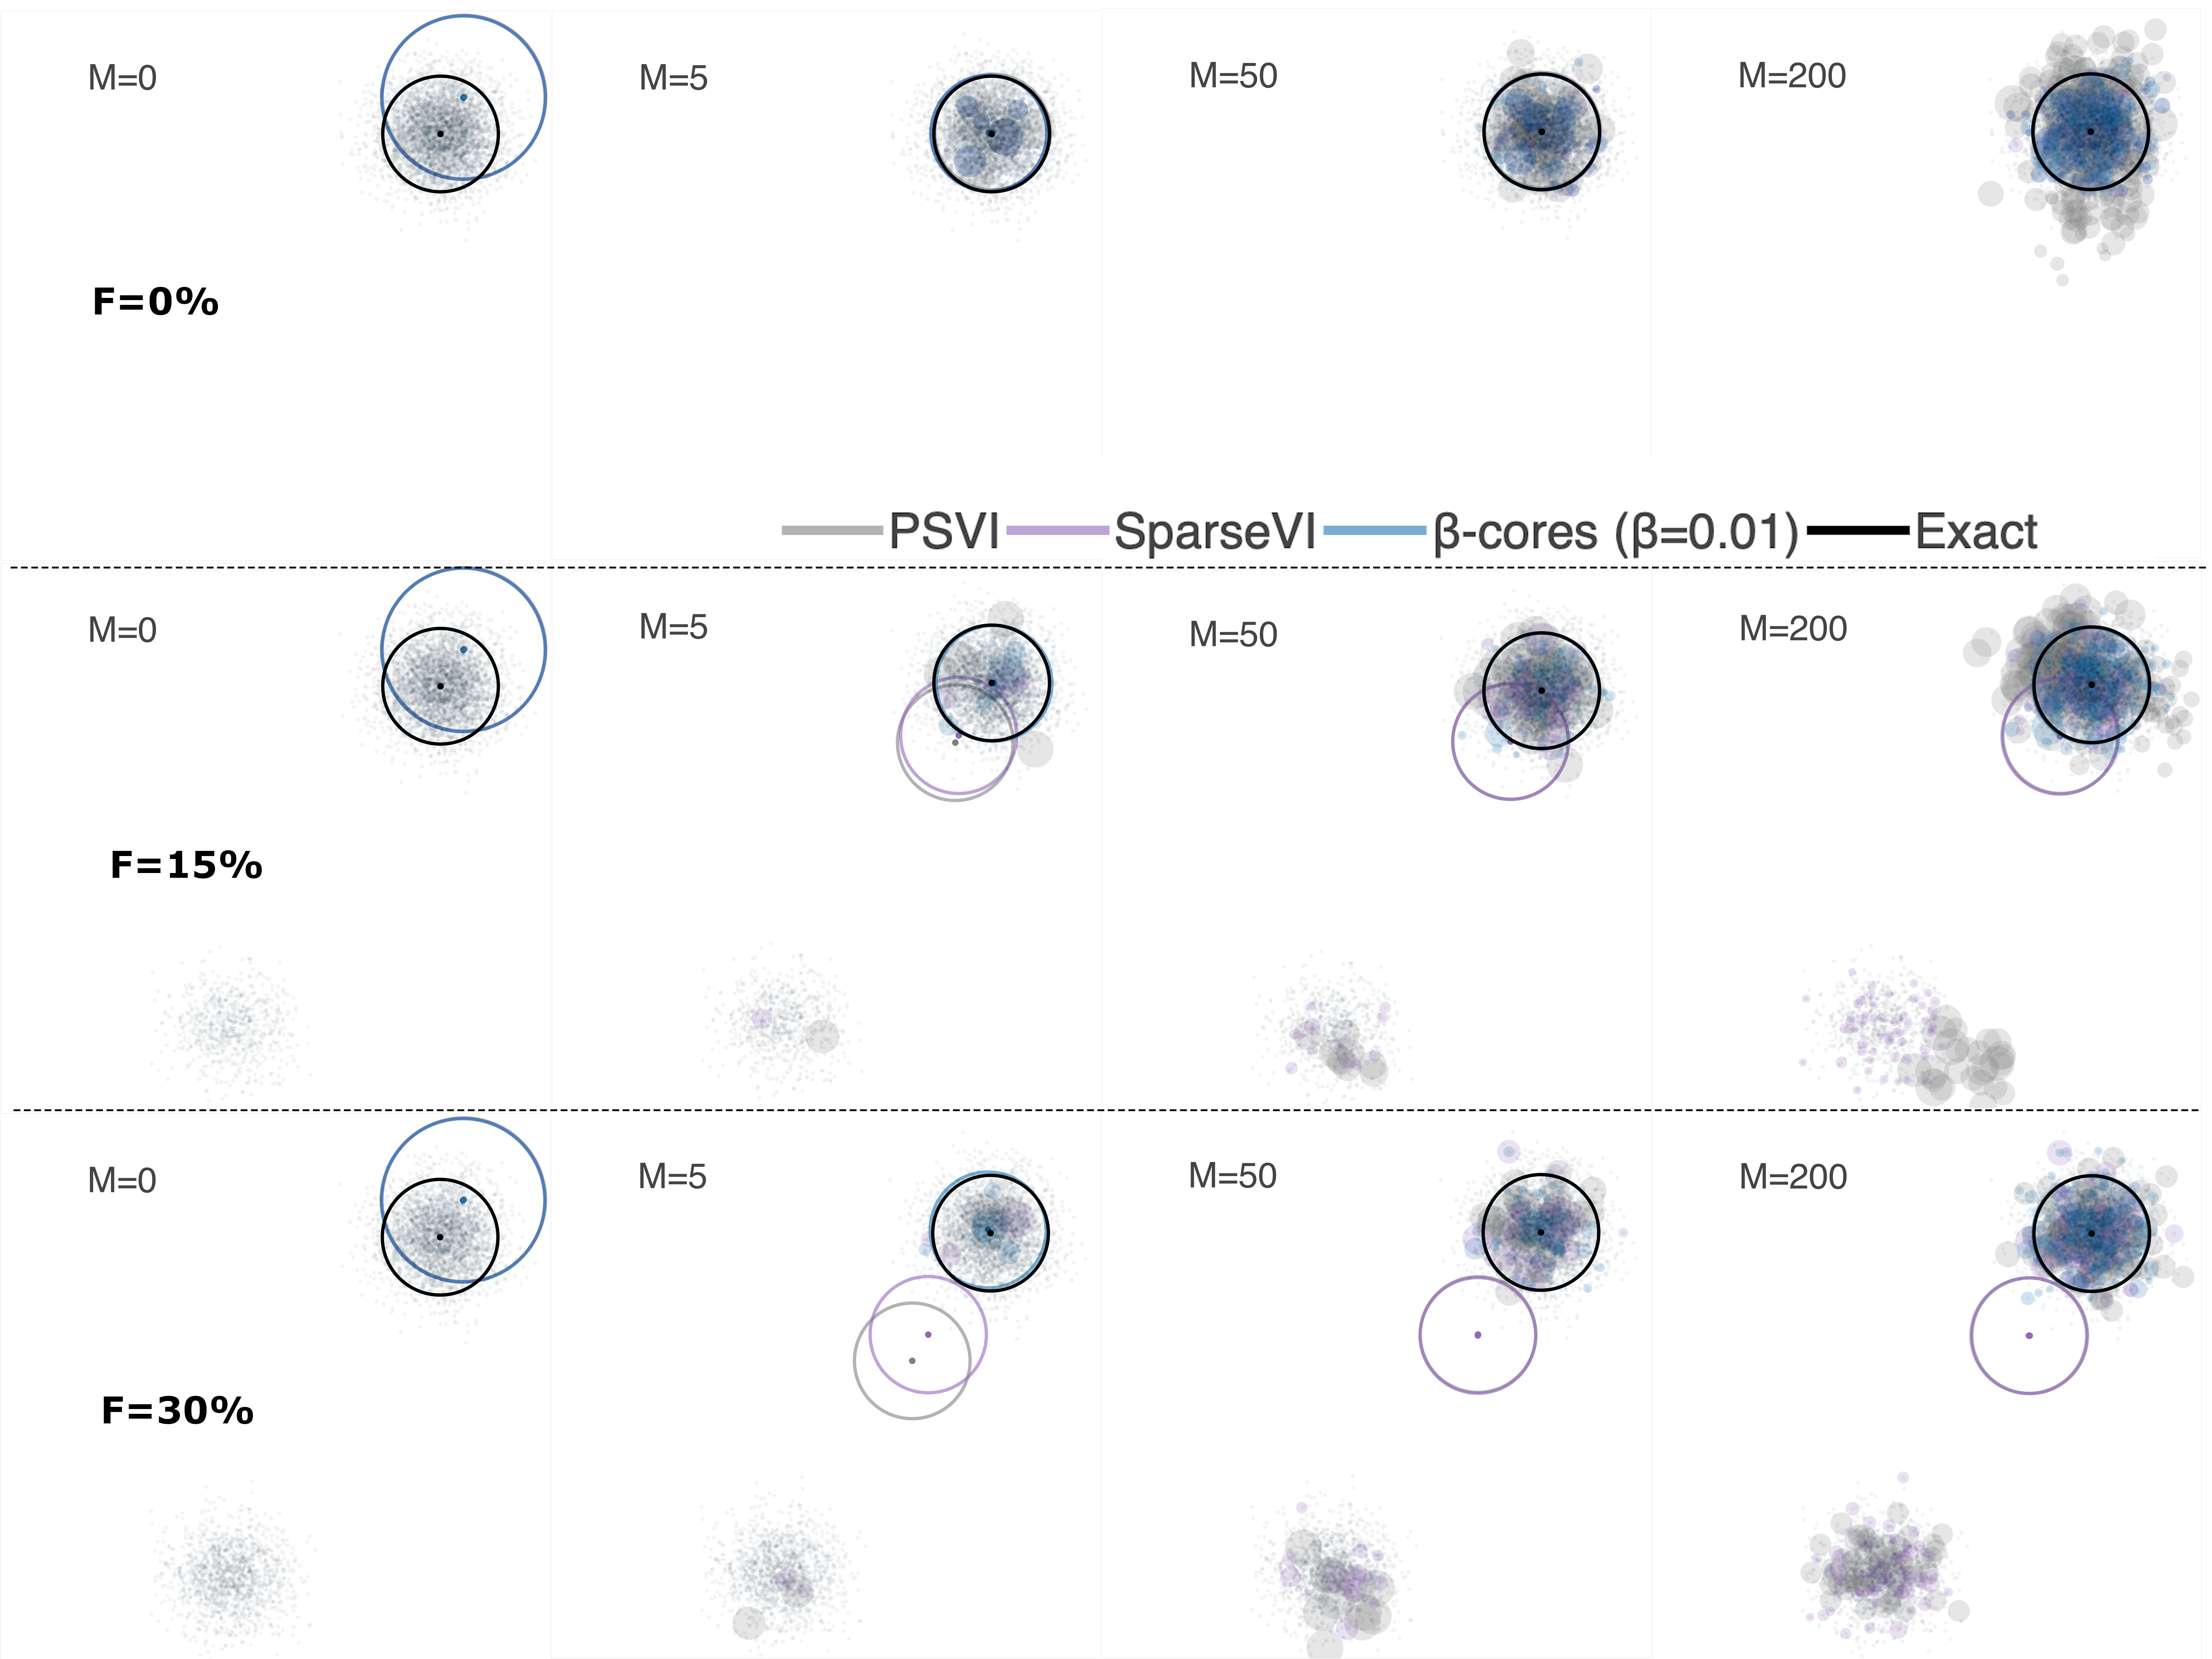
\includegraphics[width=.67\textwidth, height=4.5cm]{figs/gauss_scatterplot.png}\\
	\includegraphics[width=.3\textwidth]{figs/f0KLDvsCstSize.png}
	\includegraphics[width=.3\textwidth]{figs/f15KLDvsCstSize.png}
	\includegraphics[width=.3\textwidth]{figs/f30KLDvsCstSize.png}
\end{frame}

\begin{frame}
	\frametitle{Efficient Data Acquisition from Subpopulations for Budgeted Inference}
	\centering
	\includegraphics[width=.49\textwidth]{figs/group_diabetes06_10_01_False_ACCvsit.png}
	\includegraphics[width=.49\textwidth]{figs/group_diabetes06_10_01_False_ACCvssz.png}
	\includegraphics[width=.49\textwidth]{figs/group_diabetes06_10_0_False_ACCvsit.png}
	\includegraphics[width=.49\textwidth]{figs/group_diabetes06_10_0_False_ACCvssz.png}	
\end{frame}


\begin{frame}
	\Large{\textbf{Thanks} \\ email \href{mailto:dm754@cam.ac.uk}{dm754@cam.ac.uk}  }
	\begin{itemize}
		\item \textbf{Collaborators}: Cecilia Mascolo, Trevor Campbell, Alastair R. Beresford
		\item \textbf{Sponsors}: Nokia Bell Labs, Lundgren Fund, Darwin College Cambridge, Department of Computer Science \& Technology
	\end{itemize}
\end{frame}

\begin{comment}
\begin{frame}[allowframebreaks]{References}
	\tiny %\scriptsize
	\bibliography{references.bib}
\end{frame}
\end{comment}


\end{document}